\chapter{Módulo de Autenticación y Control de Roles} \label{chp:autenticacion}

Este capítulo está dedicado a describir y explicar el desarrollo de la parte de autenticación del sistema, detallando el control de roles de usuario, la gestión de permisos, el diseño de la pantalla principal y cómo se estructuran los datos de registro dividiéndolos entre el servicio de autenticación y la base de datos documental.

\section{Pantalla Principal y Opciones de Usuario}

Una vez que el usuario inicia sesión de manera exitosa, entrará directamente en su página de inicio o ``homePage''. En este panel se mostrarán los datos principales del perfil autenticado, tales como el nombre y los permisos que posee. Además, desde aquí se tendrá acceso a diferentes botones y funcionalidades, cuya visibilidad estará condicionada en función de los permisos del usuario.


A continuación, se muestra una imagen de la pantalla de inicio de sesión de la aplicación, donde se pueden observar los campos para introducir el correo electrónico y la contraseña, así como el botón de inicio de sesión:
\begin{figure}[H]
    \centering
    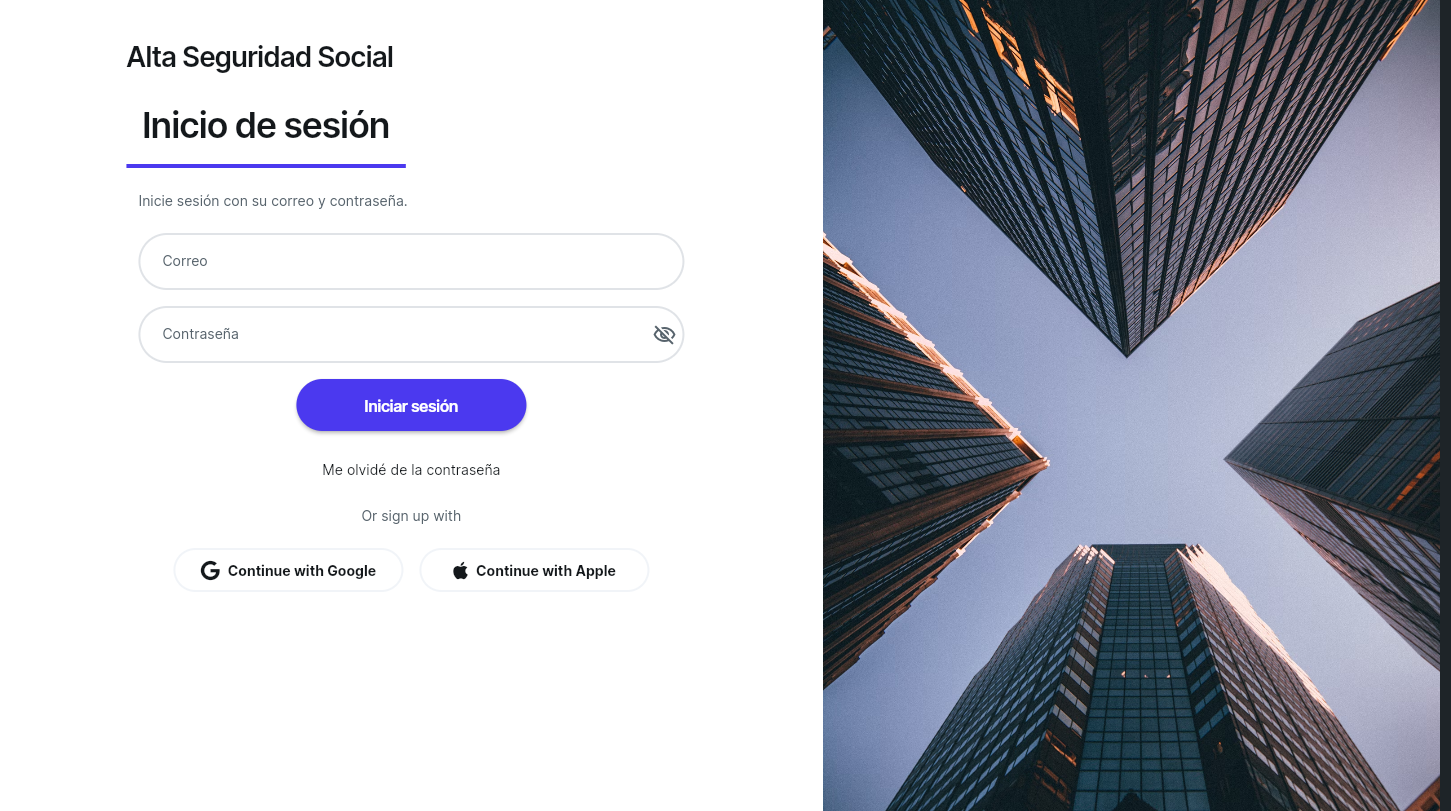
\includegraphics[width=0.8\textwidth]{imagenes/05_Login.png}
    \caption{Pantalla de inicio de sesión}
\end{figure}

La página está compuesta por un formulario sencillo. Como bien se ha mencionado en el apartado 4.1, no se hacen validaciones de formato en tiempo real porque dichas validaciones se harán a través del formulario de creación de usuarios.
\subsection{Opciones de Administrador}

Los usuarios que cuenten con el rol de administrador dispondrán de capacidades de gestión de entidades y personal, teniendo acceso a las siguientes opciones:
\begin{itemize}
    \item \textbf{Dar de alta a empresas:} El administrador, mediante un formulario para recoger todos los datos necesarios de la entidad, podrá dar de alta a nuevas empresas en la aplicación para que estas puedan usar el servicio.
    \item \textbf{Dar de alta a usuarios:} El administrador también podrá registrar a un nuevo usuario para que este pueda, de forma exclusiva para la empresa o empresas seleccionadas, dar de alta a nuevos empleados.
\end{itemize}

\subsection{Opciones de Supervisor}

Los usuarios con el rol de supervisor tendrán acceso a las mismas opciones que los administradores, pero con una limitación importante: solo podrán dar de alta a nuevos usuarios de recursos humanos (RRHH) dentro de su ámbito de acceso autorizado. Es decir, un supervisor no podrá registrar a nuevos administradores ni modificar los permisos de acceso a empresas, pero sí podrá gestionar la creación de perfiles operativos de RRHH para facilitar la administración interna de la empresa o empresas a las que tiene acceso autorizado. Este es el rol que tendrán dentro de la aplicación los gestores de las gestorías, ya que podrán gestionar a su vez a los usuarios de RRHH de sus clientes, pero no tendrán acceso a la gestión de empresas ni a la creación de administradores globales del sistema.

Esta delegación de permisos permite una gestión más eficiente y segura del sistema, evitando que se otorguen privilegios excesivos a usuarios que no necesitan acceso completo a la plataforma.


\subsection{Opciones del Usuario de Recursos Humanos}

Por otro lado, los usuarios de recursos humanos (RRHH) tendrán acceso a las operativas de registro de trabajadores, divididas en las siguientes acciones: \begin{itemize} \item \textbf{Seleccionar empresa:} De entre todas las empresas a las que el usuario de RRHH tiene acceso autorizado, este deberá escoger aquella en la que quiera tramitar un alta. \item \textbf{Dar de alta:} Una vez escogida la empresa, se procederá a recoger los datos personales y contractuales necesarios del empleado para formalizar su registro. \end{itemize}



\section{Gestión de Datos y Formulario Dual}

Para dar de alta a un usuario (o empleado), el administrador debe rellenar un formulario específico. Este formulario va a tener una doble función arquitectónica, debido a que el servicio de Google Auth no permite añadir campos personalizados adicionales al perfil básico. Por un lado, se guardarán los datos de acceso en Google Auth (estos son el correo y el hash de la contraseña), garantizando la encriptación de la contraseña; por otro lado, el resto de los campos operativos se guardarán dentro de la base de datos Firestore bajo la colección \textit{users}.

\subsection{Almacenamiento en Google Auth}

A la plataforma de autenticación de Google se enviarán exclusivamente los datos críticos de acceso:
\begin{itemize}
    \item \textbf{Correo}: El correo electrónico del usuario, que se utilizará como identificador para el inicio de sesión.
    \item \textbf{Hash de contraseña}: La contraseña del usuario, que se almacenará de forma segura y cifrada por Google Auth, garantizando la protección de esta información sensible.
\end{itemize}
Es importante recalcar que, aunque el correo se almacena en Google Auth, este mismo dato también se guarda en la base de datos documental (Firestore) para poder realizar las validaciones de permisos y roles de manera eficiente.

Sin embargo, la contraseña no se almacena en Google Auth, sino que se guarda un ``resumen'' o ``hash'' de la misma con técnicas de cifrado avanzadas (bcrypt), lo que garantiza que incluso en caso de una brecha de seguridad, las contraseñas de los usuarios no puedan ser recuperadas ni utilizadas por terceros malintencionados.

Además, dos contraseñas idénticas de diferentes usuarios no tendrán el mismo hash, porque se utiliza un proceso de salting que añade un valor aleatorio a cada contraseña antes de cifrarla, lo que aumenta significativamente la seguridad del sistema de autenticación.

En su lugar, Google Auth devuelve un token de sesión cifrado y un identificador único (UID) que se utilizan para vincular el perfil de autenticación con el documento de permisos en Firestore, garantizando así una gestión segura y eficiente de los datos de acceso.
Esto se usará para validar el acceso a la aplicación y para gestionar los permisos de cada usuario, asegurando que solo aquellos con las credenciales correctas puedan acceder a las funcionalidades correspondientes a su rol.

A continuación, se muestran dos imágenes (una de Google Auth y otra de Firestore), una por encima de la otra, para ilustrar cómo se dividen los datos entre ambos servicios y cómo se complementan para ofrecer una solución de autenticación robusta y segura, omitiendo por motivos de seguridad algunos campos:
\begin{figure}[H]
    \centering
    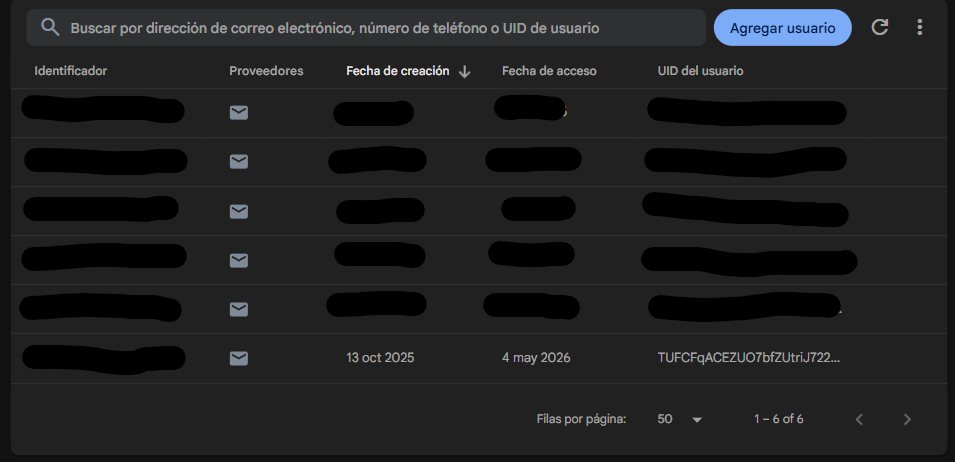
\includegraphics[width=0.8\textwidth]{imagenes/05_GoogleAuth.png}
    \caption{Datos almacenados en Google Auth}
\end{figure}
\begin{figure}[H]
    \centering
    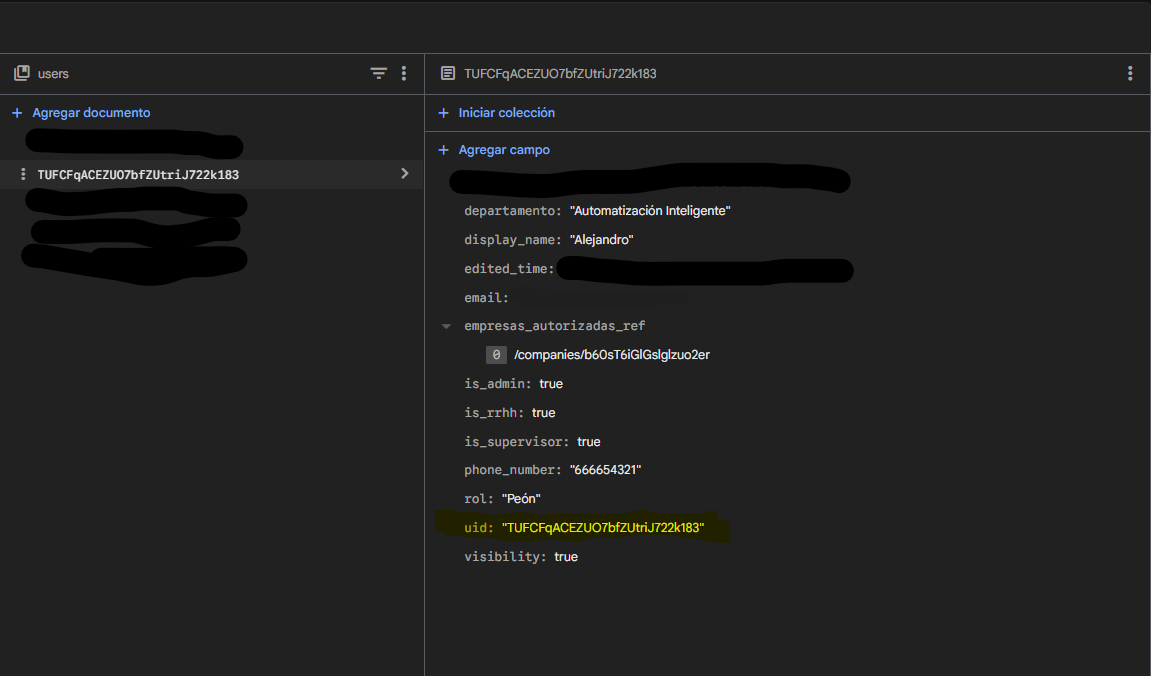
\includegraphics[width=0.8\textwidth]{imagenes/05_Firestore.png}
    \caption{Datos almacenados en Firestore}
\end{figure}

\subsection{Almacenamiento en Firestore}

Toda la información adicional y el control de roles se gestiona como documentos en la base de datos NoSQL Firestore.

Se almacena un documento por cada usuario registrado, el cual contiene campos específicos para identificar su rol (administrador, RRHH, supervisor) y las empresas a las que tiene acceso autorizado. Este enfoque permite una gestión flexible y escalable de los permisos, ya que se pueden añadir o modificar campos sin afectar la estructura general de la base de datos. Además, se implementan índices compuestos para optimizar las consultas y garantizar que los usuarios solo puedan acceder a la información de las empresas que tienen autorizadas, manteniendo así la seguridad y privacidad de los datos.
Esto último es especialmente importante para cumplir con el RGPD, ya que garantiza que los datos de cada empresa estén segregados y solo accesibles para los usuarios autorizados, evitando cualquier riesgo de acceso no autorizado o violación de la privacidad.

A continuación, se muestra una imagen del formulario de registro de un nuevo usuario, donde se pueden observar los campos que se rellenan para almacenar la información tanto en Google Auth como en Firestore:
\begin{figure}[H]
    \centering
    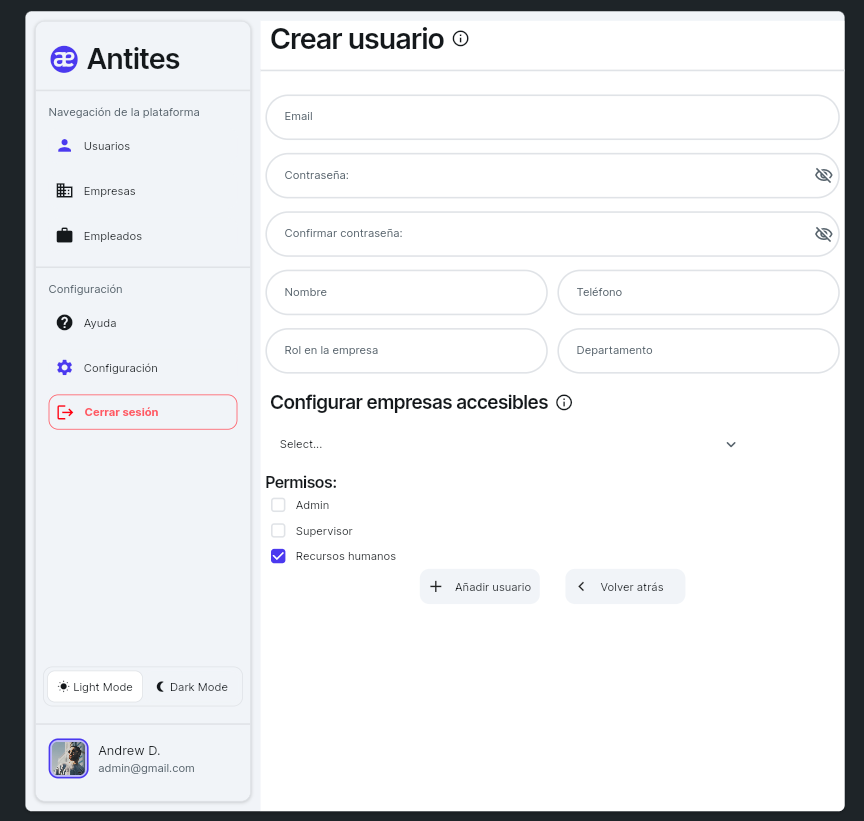
\includegraphics[width=0.8\textwidth]{imagenes/05_FormularioRegistro.png}
    \caption{Formulario de registro de un nuevo usuario}
\end{figure}

Como se puede observar en la imagen, el formulario recoge tanto los datos de acceso (correo y contraseña) que se envían a Google Auth, como los datos adicionales (rol y empresas autorizadas) que se almacenan en Firestore. Esta estructura dual permite una gestión eficiente y segura de la autenticación y los permisos de los usuarios dentro de la plataforma.

Además, se puede observar que la casilla de ``Recursos humanos'' está marcada por defecto, al contrario que las de ``Administrador'' y ``Supervisor'', que están desmarcadas. Esto se debe a que, en la mayoría de los casos, el perfil de RRHH es el más común entre los usuarios de la plataforma, mientras que los roles de administrador y supervisor suelen ser más limitados y específicos. A pesar de ello, por ser una casilla de tipo checkbox, el administrador tiene la libertad de marcar o desmarcar cualquiera de las opciones según las necesidades de cada usuario registrado.

\subsubsection{Campos de Identificación y Roles}

Dentro del documento de cada usuario en Firestore se almacenan los siguientes campos:

\begin{itemize}
    \item \textbf{Correo:} El mismo correo que se usará para el inicio de sesión, actuando como identificador común.
    \item \textbf{Is\_admin:} Un campo lógico (cierto o falso). Se utilizará para autorizar la vista u oculte de botones a los que un usuario de la aplicación puede acceder.
    \item \textbf{Is\_rrhh:} Un campo de valor lógico similar al anterior, que identifica a los usuarios operativos de recursos humanos.
    \item \textbf{Is\_supervisor:} El tercer campo de valor cierto o falso. Aquellos usuarios con este campo con valor cierto tendrán privilegios para registrar a otros usuarios de RRHH dentro de su ámbito.
\end{itemize}
\subsubsection{Control de Acceso Multi-Tenant}
Para garantizar la segregación de la información de las distintas organizaciones, se utiliza un campo adicional: \begin{itemize} \item \textbf{Empresas autorizadas:} Un campo estructural que se utilizará para gestionar e identificar a qué empresas específicas tiene acceso un usuario. \end{itemize}

\subsubsection{Lista de datos de un usuario}
A continuación, se muestra una lista con todos los campos que se almacenan en el documento de cada usuario en Firestore, incluyendo el tipo de dato y su función dentro del sistema de autenticación y control de roles:
\begin{itemize}
    \item \textbf{Correo (String): } El correo electrónico del usuario, que también se almacena en Google Auth para la autenticación.
    \item \textbf{UID (String)} El identificador único que devuelve Google Auth, utilizado para vincular el perfil de autenticación con el documento de permisos en Firestore.
    \item \textbf{Created\_time (Timestamp):} La fecha y hora en que se creó el usuario, útil para auditorías y gestión de usuarios.
    \item \textbf{Edited\_time (Timestamp):} La fecha y hora de la última modificación del perfil del usuario, para mantener un registro actualizado. Este campo no aparecerá en el fichero hasta que no se modifique el perfil por primera vez.
    \item \textbf{Phone\_number (String):} Un campo opcional para almacenar el número de teléfono del usuario, que puede ser utilizado para comunicaciones internas o autenticación de dos factores.
    \item \textbf{is\_admin (Boolean):} Explicado anteriormente.
    \item \textbf{is\_rrhh (Boolean):} Idem al anterior, pero para identificar a los usuarios de recursos humanos.
    \item \textbf{is\_supervisor (Boolean):} Idem al anterior, pero para identificar a los usuarios con privilegios de supervisión.
    \item \textbf{Empresas\_autorizadas\_ref (Vector de referencias de empresas):} Un campo estructural (array) que contiene referencias a los documentos de las empresas a las que el usuario tiene acceso autorizado, utilizado para gestionar el control de acceso multi-tenant.
    \item \textbf{Rol (String):} Un campo en el que se explica cuál es la función del usuario dentro de la empresa, como por ejemplo ``Jefe de RRHH'', ``Supervisor de nóminas'', etc. Este campo es meramente informativo y no se utiliza para la gestión de permisos, pero puede ser útil para identificar el perfil profesional del usuario dentro de la organización.
    \item \textbf{Departamento (String):} Similar al campo de rol, este campo describe a qué departamento pertenece el usuario dentro de la empresa, como por ejemplo ``Recursos Humanos'', ``Finanzas'', etc. Al igual que el campo de rol, es un dato informativo que no afecta a la gestión de permisos, pero puede ser útil para segmentar y organizar a los usuarios dentro de la plataforma.
    \item \textbf{Visibility (Boolean):} Un campo lógico que se utiliza para controlar la visibilidad del perfil del usuario dentro de la plataforma. Si este campo tiene un valor de falso, el perfil del usuario no será visible para otros usuarios, lo que puede ser útil para gestionar usuarios inactivos o para mantener la privacidad de ciertos perfiles dentro de la organización. Esto se usa para ``borrar'' usuarios sin eliminar completamente su información de la base de datos, garantizando la trazabilidad y la integridad de los datos, cumpliendo así con las normativas de protección de datos y facilitando la gestión de usuarios a largo plazo. 
\end{itemize}

\section{Cumplimiento del RGPD y Asignación Manual}

El flujo de asignación de empresas a los usuarios conlleva un protocolo estricto. Inicialmente, se dará de alta a un usuario manualmente, dejando vacío el campo de empresas autorizadas. Una vez que el usuario ha sido registrado exitosamente, es el superusuario encargado del control y mantenimiento de este servicio quien debe añadir manualmente el identificador (ID) de la empresa o empresas a las que este usuario tiene acceso.

Este procedimiento debe realizarse obligatoriamente de esta manera para garantizar que no se viole el Reglamento General de Protección de Datos (RGPD). De no seguirse este control estricto, cualquier administrador podría dar acceso a un usuario a los datos confidenciales de otra compañía (como, por ejemplo, la empresa de la competencia). En pocas palabras, el dato ``Empresas autorizadas'' es un dato exclusivo de backend, protegido contra asignaciones automáticas no verificadas.

Una vez que el superusuario ha asignado manualmente el acceso a las empresas correspondientes, se consideran dos escenarios posibles para los usuarios de RRHH, dependiendo de si tienen o no el campo `Is\_supervisor` con valor cierto o falso:
\begin{itemize}
    \item \textbf{Is\_supervisor = true:} Si el usuario tiene el campo `Is\_supervisor` con valor cierto, tendrá privilegios para registrar a otros usuarios de RRHH dentro de su ámbito. Es decir, podrá dar de alta a nuevos usuarios de RRHH y asignarles el mismo acceso a empresas que él tiene autorizado, pero no podrá modificar los permisos de acceso a empresas ni asignar permisos de administrador.
    \item \textbf{Is\_supervisor = false:} Si el usuario no tiene el campo `Is\_supervisor` con valor cierto, entonces este usuario no tendrá privilegios para registrar a otros usuarios de RRHH dentro de su ámbito. Solo podrá acceder a las funcionalidades operativas de recursos humanos, como dar de alta a empleados dentro de las empresas a las que tiene acceso autorizado, pero no podrá gestionar ni asignar permisos a otros usuarios.
\end{itemize}
